%% Преамбула TeX-файла

% 1. Стиль и язык
\documentclass[utf8x, 12pt]{G7-32} % Стиль (по умолчанию будет 14pt)

% Остальные стандартные настройки убраны в preamble.inc.tex.
\sloppy

% Настройки стиля ГОСТ 7-32
% Для начала определяем, хотим мы или нет, чтобы рисунки и таблицы нумеровались в пределах раздела, или нам нужна сквозная нумерация.
\EqInChapter % формулы будут нумероваться в пределах раздела
\TableInChapter % таблицы будут нумероваться в пределах раздела
\PicInChapter % рисунки будут нумероваться в пределах раздела
\usepackage{slashbox}

% Добавляем гипертекстовое оглавление в PDF
\usepackage[
bookmarks=true, colorlinks=true, unicode=true,
urlcolor=black,linkcolor=black, anchorcolor=black,
citecolor=black, menucolor=black, filecolor=black,
]{hyperref}

% Изменение начертания шрифта --- после чего выглядит таймсоподобно.
% apt-get install scalable-cyrfonts-tex

\IfFileExists{cyrtimes.sty}
    {
        \usepackage{cyrtimespatched}
    }
    {
        % А если Times нету, то будет CM...
    }

\usepackage{graphicx}   % Пакет для включения рисунков

% С такими оно полями оно работает по-умолчанию:
% \RequirePackage[left=20mm,right=10mm,top=20mm,bottom=20mm,headsep=0pt]{geometry}
% Если вас тошнит от поля в 10мм --- увеличивайте до 20-ти, ну и про переплёт не забывайте:
\geometry{right=20mm}
\geometry{left=30mm}


% Пакет Tikz
\usepackage{tikz}
\usetikzlibrary{arrows,positioning,shadows}

% Произвольная нумерация списков.
\usepackage{enumerate}

% ячейки в несколько строчек
\usepackage{multirow}

% itemize внутри tabular
\usepackage{paralist,array}

% Центрирование подписей к плавающим окружениям
\usepackage[justification=centering]{caption}

% объявляем новую команду для переноса строки внутри ячейки таблицы
\newcommand{\specialcell}[2][c]{%
	\begin{tabular}[#1]{@{}c@{}}#2\end{tabular}}



% Настройки листингов.
\ifPDFTeX
% Листинги

\usepackage{listings}
\usepackage{wrapfig}
% Значения по умолчанию
\lstset{
  basicstyle= \footnotesize,
  breakatwhitespace=true,% разрыв строк только на whitespacce
  breaklines=true,       % переносить длинные строки
%   captionpos=b,          % подписи снизу -- вроде не надо
  inputencoding=koi8-r,
  numbers=left,          % нумерация слева
  numberstyle=\footnotesize,
  showspaces=false,      % показывать пробелы подчеркиваниями -- идиотизм 70-х годов
  showstringspaces=false,
  showtabs=false,        % и табы тоже
  stepnumber=1,
  tabsize=4,              % кому нужны табы по 8 символов?
  frame=single,
  escapeinside={(*}{*)}, %выделение
  literate={а}{{\selectfont\char224}}1
  {б}{{\selectfont\char225}}1
  {в}{{\selectfont\char226}}1
  {г}{{\selectfont\char227}}1
  {д}{{\selectfont\char228}}1
  {е}{{\selectfont\char229}}1
  {ё}{{\"e}}1
  {ж}{{\selectfont\char230}}1
  {з}{{\selectfont\char231}}1
  {и}{{\selectfont\char232}}1
  {й}{{\selectfont\char233}}1
  {к}{{\selectfont\char234}}1
  {л}{{\selectfont\char235}}1
  {м}{{\selectfont\char236}}1
  {н}{{\selectfont\char237}}1
  {о}{{\selectfont\char238}}1
  {п}{{\selectfont\char239}}1
  {р}{{\selectfont\char240}}1
  {с}{{\selectfont\char241}}1
  {т}{{\selectfont\char242}}1
  {у}{{\selectfont\char243}}1
  {ф}{{\selectfont\char244}}1
  {х}{{\selectfont\char245}}1
  {ц}{{\selectfont\char246}}1
  {ч}{{\selectfont\char247}}1
  {ш}{{\selectfont\char248}}1
  {щ}{{\selectfont\char249}}1
  {ъ}{{\selectfont\char250}}1
  {ы}{{\selectfont\char251}}1
  {ь}{{\selectfont\char252}}1
  {э}{{\selectfont\char253}}1
  {ю}{{\selectfont\char254}}1
  {я}{{\selectfont\char255}}1
  {А}{{\selectfont\char192}}1
  {Б}{{\selectfont\char193}}1
  {В}{{\selectfont\char194}}1
  {Г}{{\selectfont\char195}}1
  {Д}{{\selectfont\char196}}1
  {Е}{{\selectfont\char197}}1
  {Ё}{{\"E}}1
  {Ж}{{\selectfont\char198}}1
  {З}{{\selectfont\char199}}1
  {И}{{\selectfont\char200}}1
  {Й}{{\selectfont\char201}}1
  {К}{{\selectfont\char202}}1
  {Л}{{\selectfont\char203}}1
  {М}{{\selectfont\char204}}1
  {Н}{{\selectfont\char205}}1
  {О}{{\selectfont\char206}}1
  {П}{{\selectfont\char207}}1
  {Р}{{\selectfont\char208}}1
  {С}{{\selectfont\char209}}1
  {Т}{{\selectfont\char210}}1
  {У}{{\selectfont\char211}}1
  {Ф}{{\selectfont\char212}}1
  {Х}{{\selectfont\char213}}1
  {Ц}{{\selectfont\char214}}1
  {Ч}{{\selectfont\char215}}1
  {Ш}{{\selectfont\char216}}1
  {Щ}{{\selectfont\char217}}1
  {Ъ}{{\selectfont\char218}}1
  {Ы}{{\selectfont\char219}}1
  {Ь}{{\selectfont\char220}}1
  {Э}{{\selectfont\char221}}1
  {Ю}{{\selectfont\char222}}1
  {Я}{{\selectfont\char223}}1
}

% Стиль для псевдокода: строчки обычно короткие, поэтому размер шрифта побольше
\lstdefinestyle{pseudocode}{
  basicstyle=\small,
  keywordstyle=\color{black}\bfseries\underbar,
  language=Pseudocode,
  numberstyle=\footnotesize,
  commentstyle=\footnotesize\it
}

% Стиль для обычного кода: маленький шрифт
\lstdefinestyle{realcode}{
  basicstyle=\scriptsize,
  numberstyle=\footnotesize
}

% Стиль для коротких кусков обычного кода: средний шрифт
\lstdefinestyle{simplecode}{
  basicstyle=\footnotesize,
  numberstyle=\footnotesize
}

% Стиль для BNF
\lstdefinestyle{grammar}{
  basicstyle=\footnotesize,
  numberstyle=\footnotesize,
  stringstyle=\bfseries\ttfamily,
  language=BNF
}

% Определим свой язык для написания псевдокодов на основе Python
\lstdefinelanguage[]{Pseudocode}[]{Python}{
  morekeywords={each,empty,wait,do},% ключевые слова добавлять сюда
  morecomment=[s]{\{}{\}},% комменты {а-ля Pascal} смотрятся нагляднее
  literate=% а сюда добавлять операторы, которые хотите отображать как мат. символы
    {->}{\ensuremath{$\rightarrow$}~}2%
    {<-}{\ensuremath{$\leftarrow$}~}2%
    {:=}{\ensuremath{$\leftarrow$}~}2%
    {<--}{\ensuremath{$\Longleftarrow$}~}2%
}[keywords,comments]

% Свой язык для задания грамматик в BNF
\lstdefinelanguage[]{BNF}[]{}{
  morekeywords={},
  morecomment=[s]{@}{@},
  morestring=[b]",%
  literate=%
    {->}{\ensuremath{$\rightarrow$}~}2%
    {*}{\ensuremath{$^*$}~}2%
    {+}{\ensuremath{$^+$}~}2%
    {|}{\ensuremath{$|$}~}2%
}[keywords,comments,strings]

% Подписи к листингам на русском языке.
\renewcommand\lstlistingname{\cyr\CYRL\cyri\cyrs\cyrt\cyri\cyrn\cyrg}
\renewcommand\lstlistlistingname{\cyr\CYRL\cyri\cyrs\cyrt\cyri\cyrn\cyrg\cyri}

\else
\usepackage{local-minted}
\fi

% Полезные макросы листингов.
% Любимые команды
\newcommand{\Code}[1]{\textbf{#1}}


\begin{document}

\frontmatter % выключает нумерацию ВСЕГО; здесь начинаются ненумерованные главы: реферат, введение, глоссарий, сокращения и прочее.

% Команды \breakingbeforechapters и \nonbreakingbeforechapters
% управляют разрывом страницы перед главами.
% По-умолчанию страница разрывается.

% \nobreakingbeforechapters
% \breakingbeforechapters

%% \begin{titlepage}
% 	\centering
% 	{\scshape\LARGE МГТУ им. Баумана \par}
% 	\vspace{3cm}
% 	{\scshape\Large Лабораторная работа №4\par}
% 	\vspace{0.5cm}
% 	{\scshape\Large По курсу: "Анализ алгоритмов"\par}
% 	\vspace{1.5cm}
% 	{\huge\bfseries Параллельное умножение матриц\par}
% 	\vspace{2cm}
% 	\Large Работу выполнила: Оберган Татьяна, ИУ7-55Б\par
% 	\vspace{0.5cm}
% 	\LargeПреподаватели:  Волкова Л.Л., Строганов Ю.В.\par

% 	\vfill
% 	\large \textit {Москва, 2019} \par
% \end{titlepage}


% НАЧАЛО ТИТУЛЬНОГО ЛИСТА
\noindent \begin{minipage}{0.15\textwidth}
	
\includegraphics[width=\linewidth]{b_logo}
\end{minipage}
\noindent\begin{minipage}{0.9\textwidth}\centering
	\textbf{Министерство науки и высшего образования Российской Федерации}\\
	\textbf{Федеральное государственное бюджетное образовательное учреждение высшего образования}\\
	\textbf{«Московский государственный технический университет имени Н.Э.~Баумана}\\
	\textbf{(национальный исследовательский университет)»}\\
	\textbf{(МГТУ им. Н.Э.~Баумана)}
\end{minipage}

\noindent\rule{18cm}{3pt}
\newline
\noindent ФАКУЛЬТЕТ $\underline{\text{«Информатика и системы управления»}}$ \newline
\noindent КАФЕДРА $\underline{\text{«Программное обеспечение ЭВМ и информационные технологии»}}$\newline


\begin{center}
	\noindent\begin{minipage}{1.2\textwidth}\centering
		\textbf{РАСЧЕТНО-ПОЯСНИТЕЛЬНАЯ ЗАПИСКА}\newline
		\textbf{К КУРСОВОМУ ПРОЕКТУ}\newline
		\textbf{На тему:}\newline
		\textbf{"Трехмерная визуализация маятника Ньютона"}\newline\newline\newline
	\end{minipage}
\end{center}




\noindent ~~Студент $\underline{\text{~~~~~~~~~~~~~~~~~~~~~~~~~~~~~~~~~Сукочева Алис~~~~~~~~~~~~~~~~~~~~~~~~~~~~~~~~~~~~~~~~~~~~~~~}}$

\noindent ~~Группа $\underline{\text{~~~~~~~~~~~~~~~~~~~~~~~~~~~~~~~~~~~~~~ИУ7-53Б~~~~~~~~~~~~~~~~~~~~~~~~~~~~~~~~~~~~~~~~~~~~~~~~~~~~}}$

\noindent ~~Название предприятия $\underline{\text{~~~~~~~~МГТУ им. Н. Э. Баумана, каф. ИУ7~~~~~~~~~~~~~~~~~~~~~~}}$\newline



\noindent\begin{tabular}{lcc}
	Студент: ~~~~~~~~~~~~~~~~~~~~~~~~~~~~~~~~~~~~~~~~~~~~~~~~~~~~~~~~ & $\underline{\text{~~~~~~~~~~~~~~~~}}$ & $\underline{\text{~~Сукочева А.~~}}$     \\
	                                                                  & \footnotesize подпись, дата           & \footnotesize Фамилия, И.О.              \\
	%& &  \\
	Преподаватель:                                                    & $\underline{\text{~~~~~~~~~~~~~~~~}}$ & $\underline{\text{~~~~Волкова Л.Л.~~~}}$ \\
	                                                                  & \footnotesize подпись, дата           & \footnotesize Фамилия, И. О.             \\
\end{tabular}


\begin{center}
	\vfill
	Москва~---~\the\year
	~г.
\end{center}

\thispagestyle{empty}
% КОНЕЦ ТИТУЛЬНОГО ЛИСТА

\tableofcontents

%\include{10-defines}
%\include{11-abbrev}

\Introduction

Физические тела, окружающие нас, обладают различными оптическими свойствами. Они, к примеру, могу отражать или пропускать световые лучи, также они могут отбрасывать тень. Эти и другие свойства нужно уметь наглядно показывать при помощи электронно-вычислительных машин. Этим и занимается компьютерная графика.

\textit{Компьютерная графика} -- представляет собой совокупность методов и способов преобразования информации в графическое представление при помощи ЭВМ. Без компьютерной графики не обходится ни одна современная программа. В течении нескольких десятилетий компьютерная графика прошла долгий путь, начиная с базовых алгоритмов, таких как вычерчивание линий и отрезков, до построения виртуальной реальности. 

Целью данной практики является разработка аналитической части проекта по дисциплине компьютерная графика на тему "визуализация маятника Ньютона".

В рамках выполнения работы необходимо решить следующие задачи:
\begin{enumerate}
	\item Описать предметную область работы. 
	\item Рассмотреть существующие алгоритмы построения реалистичных изображений. 
	\item Выбрать и обосновать выбор реализуемых методов или алгоритмов. 
	% 0\item Подробно изучить выбранный алгоритм.
	%\item Разработать программу на основе одного из существующих алгоритмов. Программа должна соответствовать техническому заданию и создавать реалистичное изображение. // Это уже не практика, а сама курсовая.
\end{enumerate}


\mainmatter % это включает нумерацию глав и секций в документе ниже

\chapter{ Аналитический раздел}
\label{cha:analysis}
\section{Постановка задачи}
В соответствии с техническим заданием в области компьютерной графики, необходимо реализовать программный продукт, предоставляющий визуализацию маятника Ньютона. Нужно определиться с выбором метода решения. Пользователь должен иметь возможность запуска и останова визуализируемой механической системы. В данной системе будут отсутствовать противодействующие силы, поэтому она будет действовать до тех пор, пока что пользователь не решит ее остановить. Полученное изображение должно четко показывать работу механической системы.

\section {Описание предметной области}
\textit{Компьютерная графика } -- занимает большой раздел в IT сфере. Она помогает решать многие задачи, актуальные в нашем времени. В компьютерной графике рассматривают обязательной задачей разработку алгоритмов визуализации трехмерных объектов \cite{bib2}. К примеру, визуализацию механических систем для демонстрации какого-то существующего явления без нужных, для данного явления, аппаратов.

\section {Описание алгоритмов}

\subsection {Некоторые теоретические сведения}

Прежде чем описывать алгоритмы, я хотела бы дать некоторые определения, чтобы читателю было проще воспринимать рассказанные ниже алгоритмы \cite{bib2,bib6}.

Алгоритмы удаления невидимых линий и поверхностей служат для определения линий ребер, поверхностей, которые видимы или невидимы для наблюдателя, находящегося в заданной точке пространства.

Решать задачу можно в пространстве:
\begin{enumerate}
	\item Объектном - мировая системе координат, высокая точность. Обобщённый подход, основанный на анализе пространства объектов, предполагает попарное сравнение положения всех объектов по отношению к наблюдателю.
	\item Изображений - в экранных координатах, системе координат, связанной с тем устройством в котором мы отображаем результат отображения (Графический дисплей).
\end{enumerate}

Под экранированием подразумевается загораживание одного объекта другим.

Под глубиной подразумевается значение координаты Z.

\subsection{Алгоритм Робертса}

Алгоритм Робертса -- решает задачу удаления невидимых линий. Работает в объектном пространстве. Он строго работает с выпуклыми телами. Если тело изначально является не выпуклым, то нужно его разбить на выпуклые составляющие. Алгоритм целиком основам на математических предпосылках, которые просты, точны и мощны \cite{bib1}.

Основные этапы:
\begin{enumerate}
	\item Подготовка исходных данных.
	\item Удаление линий, экранируемых самим телом.
	\item Удаление линий, экранируемых другими телами.
	\item Удаление линий пересечения тел, экранируемых самими телами, связанными отношением протыкания и другими телами.
\end{enumerate}

0. Подготовка исходных данных:

Для каждого тела сцены необходимо сформировать матрицу тела. Обозначают: V. Размерность: 4*n, где n - количество граней. Каждый столбец матрицы - это коэффициенты уравнения плоскости (4 коэффициента), проходящей через очередную грань тела.

Уравнение плоскости:

\begin{equation}
	Ax + By + Cz + D = 0
\end{equation}

В матричной форме выглядит следующим образом:

\begin{equation}
	[x\;y\;z\;1][P] = 0
\end{equation}

где 

\begin{equation}
	P = \left(
	\begin{array}{c}
			A \\
			B \\
			C \\
			D \\
		\end{array}
	\right)
\end{equation}

Тогда матрица тела будет выглядеть следующим образом:

\begin{equation}
	V = \left(
	\begin{array}{cccc}
			A_{1} & A_{2} & \ldots & A_{n} \\
			B_{1} & B_{2} & \ldots & B_{n} \\
			C_{1} & C_{2} & \ldots & C_{n} \\
			D_{1} & D_{2} & \ldots & D_{n}
		\end{array}
	\right)
\end{equation}

где n - количество граней.

Формирование матрицы:

Нужно найти коэффициенты каждой плоскости, проходящей через каждую грань тела. Располагая информацией о координатах 3 неколлинеарных точках, принадлежащий плоскости, можно найти коэффициенты данной плоскости. Плоскость однозначно задается 3 точками. Делим уравнение на d, при этом свободный член будет равен единице.

\begin{equation}
	{\begin{cases} 
			Ax_1 + By_1 + Cz_1 = -1 \\
			Ax_2 + By_2 + Cz_2 = -1 \\
			Ax_3 + By_3 + Cz_3 = -1 \\
		\end{cases}}
\end{equation}

Запишем в матричной форме:

\begin{equation}
	[X][C] = [D]
	\label{eq:ref1}
\end{equation}

где

\begin{equation}
	X = \left(
	\begin{array}{cccc}
			x_{1} & y_{1} & z_{1} \\
			x_{2} & y_{2} & z_{2} \\
			x_{3} & y_{3} & z_{3} \\
		\end{array}
	\right)
\end{equation}

~

\begin{equation}
	СC = \left(
	\begin{array}{c}
			A \\
			B \\
			C \\
		\end{array}
	\right)
\end{equation}

~

\begin{equation}
	D = \left(
	\begin{array}{c}
			-1 \\
			-1 \\
			-1 \\
		\end{array}
	\right)
\end{equation}

Решая уравнение (\ref{eq:ref1}), получаем значения коэффициентов уравнения плоскости: 

\begin{equation}
	[C] = [X]^{-1}[D]	
\end{equation}

Сформировав матрицу тела нужно проверить ее на корректность. 

Корректная матрица тела - это такая матрица, у которой любая точка, расположенная внутри тела, должна располагаться по положительную сторону от каждой грани тела. Т.е. при подставки координат любой точки, расположенной внутри тела в каждое из уравнение плоскостей в результате должно получаться положительное число. Если для очередной грани это условие не выполняется, то соответствующий столбец матрицы нужно умножить на -1. Чтобы не ошибиться с выбором точки, расположенной внутри матрицы тела, можно усреднить координаты всех вершин тела, либо взять полусумму координат максимальных и минимальных значений.

1. Удаление линий, экранируемых самим телом.

Для решения этой задачи нужно указать место расположения наблюдателя и направление его взгляда.

\begin{equation}
	E = |00-10|
	\label{eq:ref2}
\end{equation}

С одной стороны (\ref{eq:ref2}) это вектор взгляда наблюдателя, с другой стороны это вектор однородных координат точки, расположенной в минус бесконечности по оси z.

Для определения невидимых граней следует вектор взгляда E умножим матрицу тела V. Отрицательные компоненты полученного вектора будут соответствовать невидимым граням.

2. Удаление линий, экранируемых другими телами.

Наблюдатель находится в плюс бесконечности на оси z. Если на 1 этапе мы использовали вектор взгляда, то на 2 этапе мы используем координаты точки, в которой находится наблюдатель, обозначим как (\ref{eq:ref3}).

\begin{equation}
	g = |0010|
	\label{eq:ref3}
\end{equation}

Для определения невидимых точек ребра нужно построить луч, соединяющий точку наблюдения с точкой находящейся на ребре.
Точка будет невидимой, если луч на своем пути встречает в качестве преграды рассматриваемое тело.
Если тело является преградой, то луч должен пройти через тело.
Если луч проходит через тело, то он находится по положительную сторону от каждой грани тела.

3. Удаление линий пересечения тел, экранируемых самими телами, связанными отношением протыкания и другими телами.

Если тела связаны отношением взаимного протыкания, то образуются новые ребра, соответствующие линиям пересчения тел. Необходимо найти новые реба. Новые ребра можно получить путем соединения точек протыкания между собой. Вновь полученные ребра надо проверить на экранирование самими телами, связанными отношением протыкания. Оставшиеся видимые части ребер надо проверить на экранирование другими телами сцены.

Фактически на 3 этапе мы повторяем первые два этапа для новых ребер, которые получаются в результате протыкания тел.

~

Алгоритм Робертса хорошо применим для изображения множества выпуклых многогранников. Однако имеются недостатки: для визуализации более естественного изображения нам нужно уметь работать с тенью. В этом заключается один из недостатков. Без модификации и привлечения сторонних методов данный алгоритм не позволяет нам реализовывать тень. Также невозможно передать зеркальный эффект и преломление света.

\subsection{Алгоритм Варнока}

Алгоритм Варнока -- противоположен алгоритму Робертса. Решает задачу в пространстве изображений. Изображает видимые элементы. Единой версии алгоритма Варнока не существует. Можно рассматривать простейшую версию и более сложные версии алгоритма Варнока.

\begin{figure}[ht!]
	\centering{
		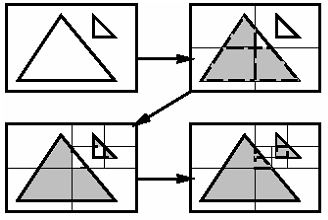
\includegraphics[width=0.5\textwidth]{img/warnock_algorithm_example2.png}
		\caption{Пример разбиения Алгоритмом Варнока}}
\end{figure}

Основная идея состоит в том, что необходимо найти ответ на вопрос о том, что изображать в очередном окне. Сначала окно имеет размеры экрана. Если мы точно не можем дать ответ, то мы окно делим на части (каждую сторону окна делим на две части). Вместо одного окна получаем 4 меньших размеров. Если снова не можем дать ответ, то продолжаем делить каждое окно на 4 части, пока не сможем дать ответ или окно не станет равным в 1 пиксель.

В простейшей версии алгоритма окно делится на подокна всякий раз, если это окно не пусто. Пределом деления является получения окна размером в 1 пиксель. Для одной точки легко определить ближайший к наблюдателю многоугольник (для этого нужно найти глубину каждого многоугольника в этой точки). В более сложных версиях делается попытка решения задачи для окон большего размера (больше одного пикселя). Для этого нужно провести классификацию многоугольников, рассматриваемых в алгоритме Варнока и действия, которые нужно предпринять в том или ином случае.

Классификация многоугольников:

\begin{enumerate}
	\item С окном связан один охватывающий многоугольник -- окно нужно закрасить цветом охватывающего многоугольника.  Рисунок \ref{fig:ref}a;
	\item С окном связан один пересекающий многоугольник -- выполняем отсечение многоугольника по границам окна и получаем один внутренний многоугольник. То есть сводим задачу к случаю с одним внутренним многоугольником.  Рисунок \ref{fig:ref}b;
	\item С окном связан один внутренний многоугольник -- окно нужно закрасить фоновым цветом, а затем выполнить растровую развертку единственного многоугольника. Рисунок \ref{fig:ref}c;
	\item Все многоугольники являются внешними по отношению к окну -- окно закрасить цветом фона.  Рисунок \ref{fig:ref}d;
\end{enumerate}

\begin{figure}[ht!]
	\centering{
		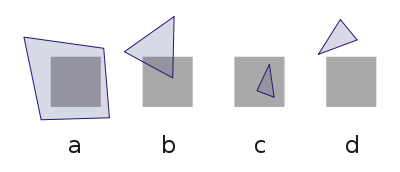
\includegraphics[width=0.6\textwidth]{img/warnock_algorithm_types.png}
		\caption{Классификация многоугольников в Алгоритме Варнока}
		\label{fig:ref}}
	
\end{figure}

К недостаткам алгоритма также можно отнести невозможность передачи зеркальных эффектов и преломления света. Также при визуализации сложной сцены число разбиений может стать очень большим, что приведет к ухудшению скорости.

\subsection{Алгоритм Вейлера-Азертона}

Алгоритм Вейлера-Азертона -- пытается минимизировать количество разбиений в алгоритме представленном выше (Алгоритме Варнока) путем разбиения окна вдоль границ многоугольника. Основой служит алгоритм Вейлера-Азертона, который используется для отсечения многоугольников.

Если многоугольники пересекают друг друга, то надо разбить один из них на два линей пересечения плоскостей присущих этим многоугольникам \cite{bib3}.

К недостаткам алгоритма относится сложность реализации, а также невозможность передачи зеркальных эффектов и преломления света.

\subsection{Алгоритм Z-буфера}

Алгоритм Z-буфера -- решает задачу в пространстве изображений. Сцены могут быть произвольной сложности, а поскольку размеры изображения ограничены размером экрана дисплея, то трудоемкость алгоритма зависит линейно от числа рассматриваемых поверхностей. Элементы сцены заносятся в буфер кадра в произвольном порядке, поэтому в данном алгоритме не тратится время на выполнение сортировок.

Буфер кадра (регенерации) - используется для заполнения атрибутов (интенсивности) каждого пикселя в пространстве изображения. Для него требуется буфер регенерации, в котором запоминаются значения яркости, а также Z-буфер (буфер глубины), куда можно помещать информацию о координате z для каждого пикселя.

Для начала нам нужно подготовить буферы. Для этого в Z-буфер заносятся максимально возможные значения z, а буфер кадра заполняется значениями пикселя, который описывает фон. Также нам нужно каждый многоугольник преобразовать в растровую форму и записать в буфер кадра. Сам процесс работы заключается в сравнении глубины каждого нового пикселя, который нужно занести в буфер кадра, с глубиной того пикселя, который уже занесён в Z-буфер. В зависимости от сравнения принимается решение, нужно ли заносить новый пиксель в буфер кадра и, если нужно, также корректируется Z-буфер (в него нужно занести глубину нового пикселя).

К недостаткам алгоритма следует отнести довольно большие объёмы требуемой памяти, а также имеются другие недостатки, которые состоят в трудоемкости устранения лестничного эффекта и трудности реализации эффектов прозрачности.

\subsection{Алгоритм прямой трассировки лучей}

Основная идея алгоритма прямой трассировки лучей состоит в том, что наблюдатель видит объекты, благодаря световым лучам, испускаемым некоторым источником, которые падают на объект, отражаются, преломляются или проходят через него и в результате достигают нас \cite{bib4}. Если проследить за лучами, то становится понятно, что среди них лишь малая часть дойдет до наблюдателя, что приведет к большим затратам ЭВМ. Заменой данному алгоритму служит метод обратный трассировки лучшей.

\subsection{Алгоритм обратной трассировки лучей}

Алгоритм обратной трассировки лучей отслеживает лучи в обратном направление (от наблюдателя к объекту). 

Считается, что наблюдатель расположен на положительной полуоси z в бесконечности, поэтому все световые лучи параллельны оси z. В ходе работы испускаются лучи от наблюдателя и ищутся пересечения луча и всех объектов сцены \cite{bib5}. В результате пересечение с максимальным значением z является видимой частью поверхности и атрибуты данного объекта используются для определения характеристик пикселя, через центр которого проходит данный световой луч. Эффективность процедуры определения пересечений луча с поверхностью объекта оказывает самое большое влияние на эффективность всего алгоритма. Чтобы избавиться от ненужного поиска пересечений было придумано искать пересечение луча с объемной оболочкой рассматриваемого объекта. Под оболочкой понимается некоторый простой объект, внутрь которого можно поместить рассматриваемый объект, к примеру параллелепипед или сфера.

\begin{figure}[ht!]
	\centering{
		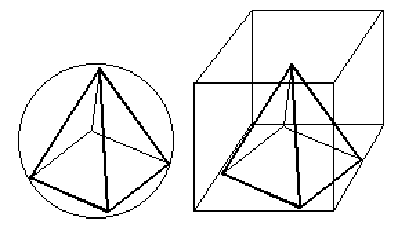
\includegraphics[width=0.6\textwidth]{img/shell.png}
		\caption{Сферическая и прямоугольная оболочки}}
\end{figure}

В дальнейшем при рассмотрении пересечения луча и объемной оболочкой рассматриваемого объекта, если такого пересечения нет, то и соответственно пересечения луча и самого рассматриваемого объекта нет, и наоборот, если мы найдем пересечение, то возможно, есть пересечение луча и рассматриваемого объекта. Для расчета эффектов освещения сцены проводятся вторичные лучи от точек пересечения ко всем источникам света. Если на пути этих лучей встречается непрозрачное тело, значит данная точка находится в тени, иначе он влияет на освещение данной точки. Также для получения более реалистичного изображения сцены, нужно учитывать вклады отраженных и преломленных лучей. 

К недостатку алгоритма относится его производительность. 
%Положительной стороной данного алгоритма является возможность использования в параллельных вычислительных системах (т.к. расчет отдельной точки выполняется независимо от других точек).

\section {Модель освещения}

Для создания реалистичного изображения в компьютерной графике применяются различные алгоритмы освещения.

Модель освещения предназначена для расчёта интенсивности
отражённого к наблюдателю света в каждой точке изображения.

Модель освещения может быть глобальной или локальной.

Локальная модель - учитывается только свет от источников и ориентация поверхности.

Локальная модель включает 3 составляющих: 

\begin{enumerate}
	\item Диффузную составляющую отражения.
	\item Отражающую составляющую отражения.
	\item Рассеянное освещение.
\end{enumerate}

Глобальная модель - учитывается ещё и свет, отражённый от других поверхностей или пропущенный через них

Глобальная модель воспроизводит чрезвычайно важные эффекты, которые будут показаны в данном проекте.

%Таким образом, глобальная модель освещения является частью алгоритмов выделения видимых поверхностей путём трассировки лучей.

\section {Вывод}

Оценив все изложенные выше алгоритмы, можно сделать вывод, что для данной работы, которая предполагает визуализацию реалистического изображения, учитывая тени, отражение объектов и тд, подходит алгоритм обратной трассировки лучей, так как он позволяет достичь высокой реалистичности построенного изображения. Он будет использоваться, несмотря на указанные недостатки, так как алгоритм достаточно полно отражает суть физических явлений с приемлемыми затратами производительности.

% Так как недостатком алгоритма обратной трассировки лучей является низкая производительность, целесообразно подумать о ее улучшении, например, реализовать его многопоточное выполнение.
\chapter{ Констукторский раздел}
\label{cha:design}


\section{Требования к программе}

Программа должна предоставлять следующие возможности:
\begin{enumerate}
	\item Визуализацию сцены.
	\item Запуск системы.
	\item Останов системы.
\end{enumerate}

\section{Выбор используемых типов и структур данных}

В данной работе нужно будет реализовать следующие типы и структуры данных.
\begin{enumerate}
	\item Точка- хранит положение, задается координатами x, y, z 
	\item Вектор - хранит направление, задается x, y, z.
	\item Сфера - хранит радиус и центр сферы, заданной точкой.
	\item Объекты на сцене - задаются сферами.
	\item Сцена - список объектов.
	\item Источник света - положение и направление света.
\end{enumerate}

\section{Алгоритм обратной трассировки лучей}
%\chapter{Технологическая часть}

\section{Выбор языка программирования и среды разработки.}

Для решения описанной заданич был выбран язык программирования - C\# \cite{Microsoft}.
Данный язык был выбран по следующим причинам.
Он использует объектно-ориентированный подход к программированию,
что позволяет работать по принципу черного ящика.
Также в языке присутствует обилие синтаксического сахара,
которое помогаем использовать готовые конструкции,
вместо того, чтобы переписывать однотипные строки кода.
Еще одним преимуществом данного языка является
наличие большого количества библиотек и шаблонов,
позволяющих не тратить время на изобретение готовых конструкций.
Стоит отменить, что данный язык является строго типизированным,
что позволяет защититься от непроконтролированных ошибок.
Также он является нативным, что необходимо
для увеличения скорости работы алгоритмов с помощью распараллеливания.

В качестве среды разработки я использовала Visual Studio Code \cite{Vs}.
Visual Studio Code подходит не только для  Windows \cite{Win},
но и для Linux \cite{Lin}, это причина,
по которой я выбрала VS code,
т.к. у меня установлена ОС Ubuntu 18.04.4 \cite{Ubuntu}.
Также моей архитектуре присутствует 8 ядер.

% \section{Сведения о модулях программы}
\section{Структура программы}

Данная программа состоит из следующих модулей:

\begin{itemize}
	\item Program.cs - файл, содержащий точку входа в программу.
	\item Vector.cs - файл, содержащий класс Vector, в котором
	      написаны основные методы для работы с вектором;
	\item Color.cs - файл, содержащий класс Color, в котором
	      написаны основные методы для работы с цветом;
	\item Constants.cs - файл, содержащий константы;
	\item Shape.cs - файл, содержащий базовый класс Shape
	      и унаследованные от него классы Sphere и Cylinder;
	\item Light.cs - файл, содержащий класс Light;
	\item MinForm.cs - файл, содержащий алгоритм трассировки лучей.
\end{itemize}

На рисунках \ref{fig:class_diagram1} - \ref{fig:class_diagram2} показана структура классов.

\begin{figure}[ht!]
	\centering{
		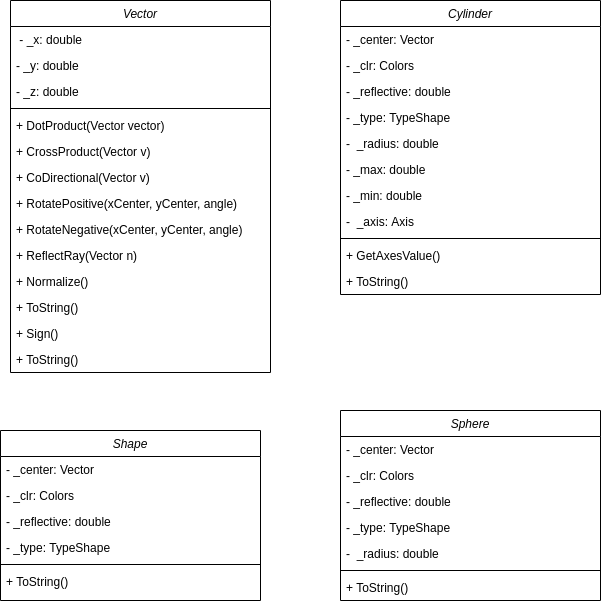
\includegraphics[width=0.75\textwidth]{class_diagram1.png}
		\caption{Структура классов}
		\label{fig:class_diagram1}}
\end{figure}

\begin{figure}[ht!]
	\centering{
		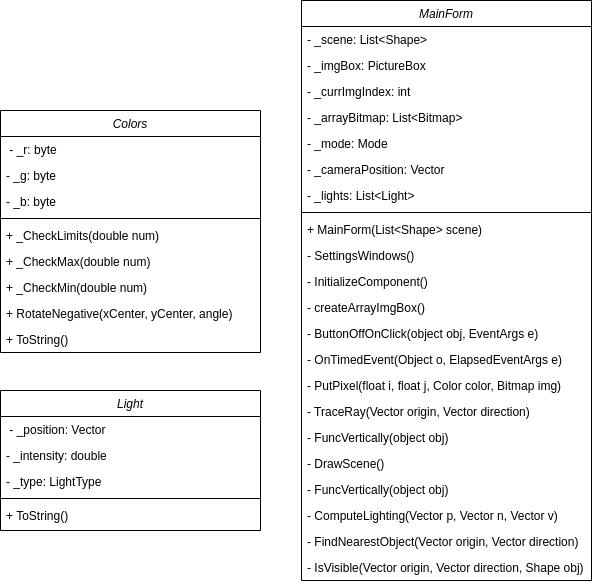
\includegraphics[width=0.75\textwidth]{class_diagram2.png}
		\caption{Структура классов}
		\label{fig:class_diagram2}}
\end{figure}

\newpage

На листинге 3.1 представлен основной код алгоритма.


\begin{lstlisting}[label=some-code,caption=Трассировка лучей.]
private Colors TraceRay(Vector origin, Vector direction, double min_t, double max_t, int depth = 3)
{
	double closest_t = Double.PositiveInfinity;
	Shape ClosestObject = FindNearestObject(origin, direction, min_t, max_t, ref closest_t);
	if (ClosestObject == null)
		return new Colors(0, 0, 0);

	Vector point = origin + direction * closest_t;
	Vector tmp = null;
	if (ClosestObject.Type == TypeShape.Sphere)
	{
		tmp = ClosestObject.Center;
	}
	else if (ClosestObject.Type == TypeShape.Cylinder)
	{
		Cylinder cylinder = ClosestObject as Cylinder;

		Vector axesValue = cylinder.GetAxesValue();   
		Vector axesValueRev = cylinder.GetAxesValue(); 		
		axesValueRev.Reverse();

		axesValue = axesValue * cylinder.Center; 
		axesValueRev = axesValueRev * point;
		tmp = axesValue + axesValueRev; 
	}

	Vector normal = point - tmp;
	normal = normal * (1.0d / normal.Length);
	Vector view = direction * -1.0d;
	double lighting = ComputeLighting(point, normal, view);

	Colors result = ClosestObject.Clr * lighting;

	if (depth <= 0)
		return result;

	Vector reflected_ray = ReflectRay(view, normal);
	Colors reflected_color = TraceRay(point, reflected_ray, 0.001d, Double.PositiveInfinity, depth - 1);

	double reflective = ClosestObject.Reflective;
	return result * (1 - reflective) + reflected_color * reflective;
}
\end{lstlisting}

\section{Вывод}

В данном разделе был выбран ЯП и среда разработки.
Также описаны модули и разобран листинг рис 3.1, показывающий работу алгоритма.
%\chapter{Экспериментальная часть}

\section{Замеры времени}

Так как одной из целью данного курсового проекта было достаточно быстрое
построение реалистичного изображения, то было применено распараллеливание
алгоритма обратной трассировки лучей.

Для замеров времени используется изображение размером 1200$\times$600.
Так как трассировка данного изображения считается достаточно короткой
задачей, используется усреднение массового эксперимента.
Сравнение произведено при n = 10.

Результат представлен на рис. \ref{ref:time}.

\begin{figure}[ht!]
	\centering{
		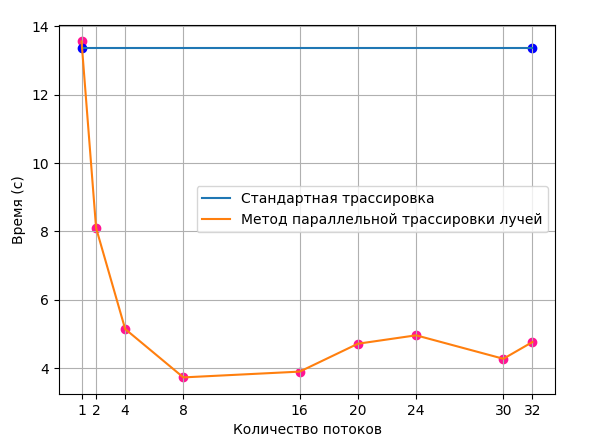
\includegraphics[width=0.7\textwidth]{time.png}
		\caption{Временные характеристики}
		\label{ref:time}}
\end{figure}

\newpage

Обычная реализация работает быстрее, чем создание одного потока,
потому что на создание потока тратится некоторое время.
При двух потоках выигрыш получается почти в два раза, так как два потока
трассируют одновременно свою часть экрана.
При увеличении числа потоков отслеживается уменьшение времени трассировки.
При 8 потоках достигается пик, при котором все ядра процессора одновременно
выполняют трассировку экрана.
Далее при увеличении числа потоков производительность падает.
Это объясняется тем, что создается очередь потоков, которая замедляет
работу программы.

\section{Вывод}

В данном разделе было произведено сравнение алгоритма трассировки лучей
при простой реализации и многопоточной (рис. \ref{ref:time}).
Результат показал, что выгоднее всего использовать все ядра процессора.


\backmatter %% Здесь заканчивается нумерованная часть документа и начинаются ссылки и
%% заключение

\Conclusion % заключение к отчёту

В результате выполнения практики была разобрана аналитическая часть работы по теме  «Реализация маятника Ньютона». Также проанализированы методы для решения этой задачи и выбран подходящий.

%%% Local Variables: 
%%% mode: latex
%%% TeX-master: "rpz"
%%% End: 


\addcontentsline{toc}{chapter}{Список литературы}
\begin{thebibliography}{3}
	\bibitem{Vs}
	Visual Studio Code [Электронный ресурс], режим доступа: https://code.visualstudio.com/ (дата обращения: 02.10.2020)
	\bibitem{Win}
	Windows [Электронный ресурс], режим доступа:https://www.microsoft.com/ru-ru/windows/ (дата обращения: 02.10.2020)
	\bibitem{Lin}
	Linux [Электронный ресурс], режим доступа:https://www.linux.org.ru/ (дата обращения: 02.10.2020)
	\bibitem{Microsoft}
	Руководство по языку C\#[Электронный ресурс], - режим доступа: https://docs.microsoft.com/ru-ru/dotnet/csharp/ (дата обращения: 02.10.2020)
	\bibitem{Ubuntu}
	Ubuntu 18.04 [Электронный ресурс], режим доступа:https://releases.ubuntu.com/18.04/ (дата обращения: 02.10.2020)
	\bibitem{tr1}
	Дымченко, Лев. Пример реализации в реальном времени метода
	трассировки лучей: необычные возможности и принцип работы. Оптимизация
	под SSE [Электронный ресурс],  режим доступа:https://www.ixbt.com/video/
	rt-raytracing.shtml. (дата обращения: 02.20.2020)
	\bibitem{tr2}
	Роджерс, Д. Алгоритмические основы машинной графики / Д. Роджерс. — Москва «Мир», 1989. — P. 512.
	\bibitem{tr3}
	Ю.М.Баяковский. Трассировка лучей из книги Джефа Проузиса [Электронный ресурс],
	режим доступа: ttps://www.graphicon.ru/oldgr/courses/cg99/notes/lect12/prouzis/raytrace.htm. (дата обращения: 02.20.2020)
\end{thebibliography}


%\appendix   % Тут идут приложения

%%\chapter{Картинки}
%\label{cha:appendix1}

%\begin{figure}
%\centering
%\caption{Картинка в приложении. Страшная и ужасная.}
%\end{figure}

%%% Local Variables: 
%%% mode: latex
%%% TeX-master: "rpz"
%%% End: 

%%\chapter{Еще картинки}
%\label{cha:appendix2}

%\begin{figure}
%\centering
%\caption{Еще одна картинка, ничем не лучше предыдущей. Но %надо же как-то заполнить место.}
%\end{figure}

%%% Local Variables: 
%%% mode: latex
%%% TeX-master: "rpz"
%%% End: 


\end{document}

%%% Local Variables:
%%% mode: latex
%%% TeX-master: t
%%% End:
